\documentclass[border=4pt]{standalone}
\usepackage{graphicx}
\usepackage{xcolor}
\usepackage{tikz}
\usetikzlibrary{arrows.meta,calc}

\definecolor{updateCyan}{HTML}{4F9FB2}
\definecolor{actionOrange}{HTML}{F59E0B}
\definecolor{feedbackGreen}{HTML}{88AD45}

\tikzset{
    module/.style={inner sep=0pt, outer sep=3pt},
    blackflow/.style={-{Latex[length=3.3mm,width=2.5mm]}, draw=black,
        line width=0.9pt},
    updateflow/.style={-{Latex[length=3.1mm,width=2.3mm]}, draw=updateCyan,
        line width=0.9pt},
    actionflow/.style={-{Latex[length=3.1mm,width=2.3mm]}, draw=actionOrange,
        line width=0.9pt},
    feedbackflow/.style={-{Latex[length=3.1mm,width=2.3mm]}, draw=feedbackGreen,
        line width=0.9pt}
}

\begin{document}
\begin{tikzpicture}
    % Observation and encoding branches.
    \node[module] (lidar) at (1.75,4.55)
        {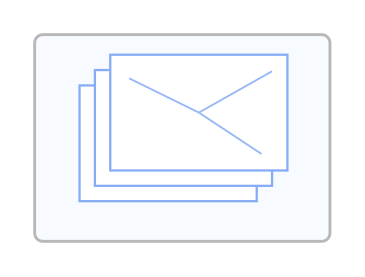
\includegraphics[width=3.00cm]{01_lidar_sequence.png}};
    \node[module] (lidarenc) at (5.85,4.55)
        {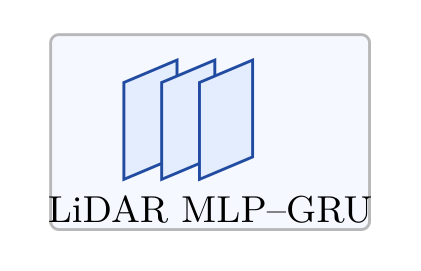
\includegraphics[width=3.55cm]{03_lidar_encoder.png}};
    \node[module] (state) at (1.75,1.30)
        {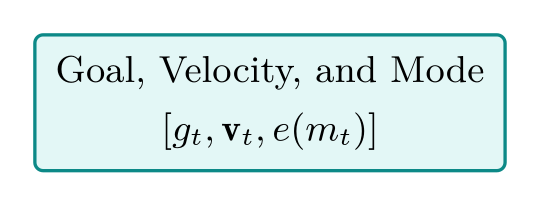
\includegraphics[width=3.55cm]{02_robot_state.png}};
    \node[module] (stateenc) at (5.85,1.30)
        {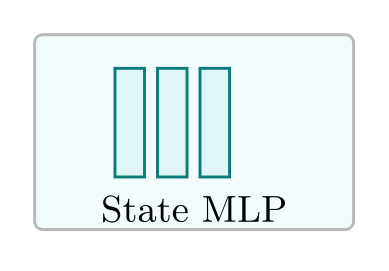
\includegraphics[width=3.55cm]{04_state_encoder.png}};
    \node[module] (fusion) at (9.20,2.90)
        {
\includegraphics[height=4.75cm]{05_fused_embedding.png}};

    % Actor, critic, and Neural-PVO heads.
    \node[module] (pvo) at (11.25,4.70)
        {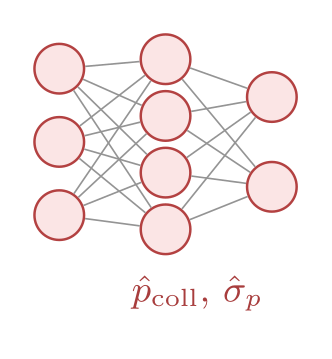
\includegraphics[width=1.45cm]{08_neural_pvo.png}};
    \node[module] (actor) at (11.25,2.72)
        {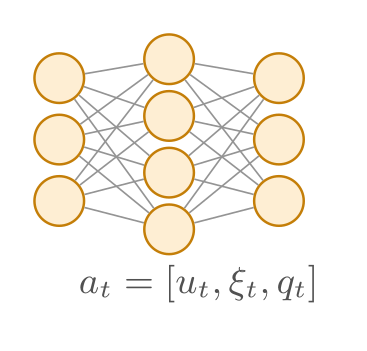
\includegraphics[width=1.45cm]{06_td3_actor.png}};
    \node[module] (critic) at (11.25,0.88)
        {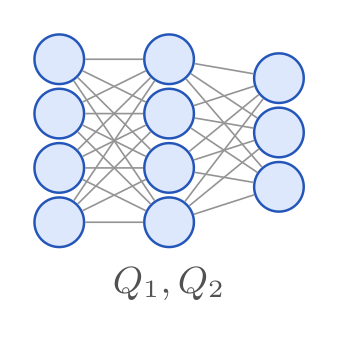
\includegraphics[width=1.45cm]{07_td3_critic.png}};

    % Risk filtering and 4WIS execution.
    \node[module] (filter) at (13.20,4.70)
        {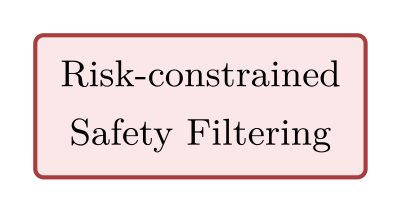
\includegraphics[width=1.50cm]{09_safety_filter.png}};
    \node[module] (mapper) at (15.12,4.70)
        {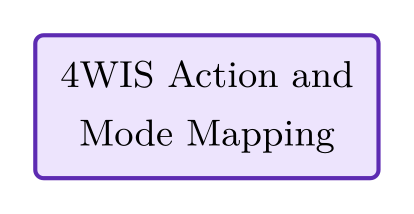
\includegraphics[width=1.58cm]{10_4wis_mapper.png}};
    \node[module] (velocity) at (17.15,4.70)
        {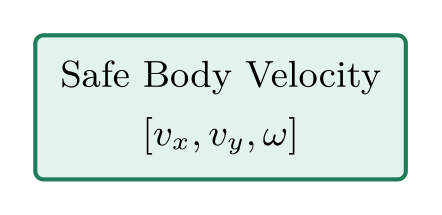
\includegraphics[width=1.72cm]{11_safe_velocity.png}};

    % Training and validation environments.
    \node[module] (irsim) at (14.10,2.30)
        {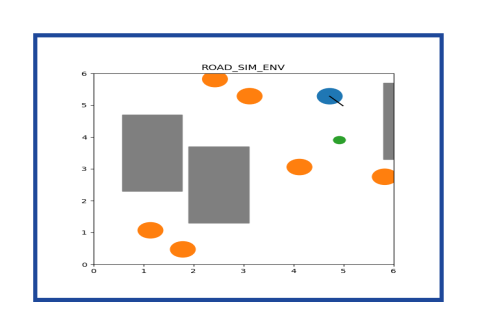
\includegraphics[width=2.45cm]{13_irsim_training.png}};
    \node[module] (reward) at (14.10,0.72)
        {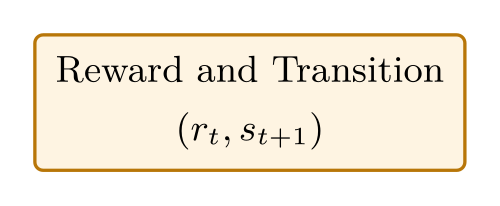
\includegraphics[width=1.85cm]{14_reward_transition.png}};
    \node[module] (gazebo) at (17.15,2.30)
        {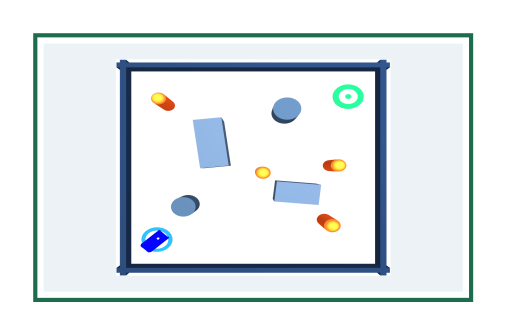
\includegraphics[width=2.55cm]{15_gazebo_validation.png}};

    % Draw all arrows after the modules so they remain visible above the PNGs.
    \draw[blackflow] (lidar.east) -- (lidarenc.west);
    \draw[blackflow] (lidarenc.east) -- (fusion.west |- lidarenc.east);
    \draw[blackflow] (state.east) -- (stateenc.west);
    \draw[blackflow] (stateenc.east) -- (fusion.west |- stateenc.east);

    \draw[blackflow] (fusion.east |- pvo.west) -- (pvo.west);
    \draw[blackflow] (fusion.east |- actor.west) -- (actor.west);
    \draw[blackflow] (fusion.east |- critic.west) -- (critic.west);

    \draw[updateflow] (critic.north) -- (actor.south);
    \draw[actionflow] (actor.north) -- (pvo.south);
    \draw[actionflow] (pvo.east) -- (filter.west);
    \draw[actionflow] (filter.east) -- (mapper.west);
    \draw[actionflow] (mapper.east) -- (velocity.west);

    \draw[actionflow] (velocity.south) -- (gazebo.north);
    \draw[actionflow] (velocity.south west) -- ++(0,-0.38) -| (irsim.north);
    \draw[feedbackflow] (irsim.south) -- (reward.north);
    \draw[feedbackflow] (reward.west) -- (critic.east);
\end{tikzpicture}
\end{document}
